\documentclass[12pt,landscape]{article}

%\usepackage{lmodern}
\usepackage{amssymb,amsmath}
\usepackage{bm}
\usepackage{graphicx}
\usepackage{microtype}
\usepackage{hyperref}
\pagestyle{empty}
\usepackage{titlesec}
\titleformat*{\section}{\LARGE\bfseries}
\titleformat*{\subsection}{\LARGE\bfseries}
\titleformat*{\subsubsection}{\LARGE\bfseries}
\setlength{\parindent}{0pt}
\setlength{\parskip}{1.2ex}
\setlength{\parindent}{0pt}
\setlength{\parskip}{1.2ex}

\setlength{\oddsidemargin}{-16mm}
\setlength{\textwidth}{260mm}
\setlength{\columnsep}{0.5in}
\setlength{\columnseprule}{1pt}
\setlength{\textheight}{202mm}
\setlength{\topmargin}{-32mm}
\setlength{\headsep}{0.25in}

\hypersetup
       {   pdfauthor = { Marco Fasondini },
           pdftitle={ foo },
           colorlinks=TRUE,
           linkcolor=black,
           citecolor=blue,
           urlcolor=blue
       }




\usepackage{upquote}
\usepackage{listings}
\usepackage{xcolor}
\lstset{
    basicstyle=\ttfamily\footnotesize,
    upquote=true,
    breaklines=true,
    breakindent=0pt,
    keepspaces=true,
    showspaces=false,
    columns=fullflexible,
    showtabs=false,
    showstringspaces=false,
    escapeinside={(*@}{@*)},
    extendedchars=true,
}
\newcommand{\HLJLt}[1]{#1}
\newcommand{\HLJLw}[1]{#1}
\newcommand{\HLJLe}[1]{#1}
\newcommand{\HLJLeB}[1]{#1}
\newcommand{\HLJLo}[1]{#1}
\newcommand{\HLJLk}[1]{\textcolor[RGB]{148,91,176}{\textbf{#1}}}
\newcommand{\HLJLkc}[1]{\textcolor[RGB]{59,151,46}{\textit{#1}}}
\newcommand{\HLJLkd}[1]{\textcolor[RGB]{214,102,97}{\textit{#1}}}
\newcommand{\HLJLkn}[1]{\textcolor[RGB]{148,91,176}{\textbf{#1}}}
\newcommand{\HLJLkp}[1]{\textcolor[RGB]{148,91,176}{\textbf{#1}}}
\newcommand{\HLJLkr}[1]{\textcolor[RGB]{148,91,176}{\textbf{#1}}}
\newcommand{\HLJLkt}[1]{\textcolor[RGB]{148,91,176}{\textbf{#1}}}
\newcommand{\HLJLn}[1]{#1}
\newcommand{\HLJLna}[1]{#1}
\newcommand{\HLJLnb}[1]{#1}
\newcommand{\HLJLnbp}[1]{#1}
\newcommand{\HLJLnc}[1]{#1}
\newcommand{\HLJLncB}[1]{#1}
\newcommand{\HLJLnd}[1]{\textcolor[RGB]{214,102,97}{#1}}
\newcommand{\HLJLne}[1]{#1}
\newcommand{\HLJLneB}[1]{#1}
\newcommand{\HLJLnf}[1]{\textcolor[RGB]{66,102,213}{#1}}
\newcommand{\HLJLnfm}[1]{\textcolor[RGB]{66,102,213}{#1}}
\newcommand{\HLJLnp}[1]{#1}
\newcommand{\HLJLnl}[1]{#1}
\newcommand{\HLJLnn}[1]{#1}
\newcommand{\HLJLno}[1]{#1}
\newcommand{\HLJLnt}[1]{#1}
\newcommand{\HLJLnv}[1]{#1}
\newcommand{\HLJLnvc}[1]{#1}
\newcommand{\HLJLnvg}[1]{#1}
\newcommand{\HLJLnvi}[1]{#1}
\newcommand{\HLJLnvm}[1]{#1}
\newcommand{\HLJLl}[1]{#1}
\newcommand{\HLJLld}[1]{\textcolor[RGB]{148,91,176}{\textit{#1}}}
\newcommand{\HLJLs}[1]{\textcolor[RGB]{201,61,57}{#1}}
\newcommand{\HLJLsa}[1]{\textcolor[RGB]{201,61,57}{#1}}
\newcommand{\HLJLsb}[1]{\textcolor[RGB]{201,61,57}{#1}}
\newcommand{\HLJLsc}[1]{\textcolor[RGB]{201,61,57}{#1}}
\newcommand{\HLJLsd}[1]{\textcolor[RGB]{201,61,57}{#1}}
\newcommand{\HLJLsdB}[1]{\textcolor[RGB]{201,61,57}{#1}}
\newcommand{\HLJLsdC}[1]{\textcolor[RGB]{201,61,57}{#1}}
\newcommand{\HLJLse}[1]{\textcolor[RGB]{59,151,46}{#1}}
\newcommand{\HLJLsh}[1]{\textcolor[RGB]{201,61,57}{#1}}
\newcommand{\HLJLsi}[1]{#1}
\newcommand{\HLJLso}[1]{\textcolor[RGB]{201,61,57}{#1}}
\newcommand{\HLJLsr}[1]{\textcolor[RGB]{201,61,57}{#1}}
\newcommand{\HLJLss}[1]{\textcolor[RGB]{201,61,57}{#1}}
\newcommand{\HLJLssB}[1]{\textcolor[RGB]{201,61,57}{#1}}
\newcommand{\HLJLnB}[1]{\textcolor[RGB]{59,151,46}{#1}}
\newcommand{\HLJLnbB}[1]{\textcolor[RGB]{59,151,46}{#1}}
\newcommand{\HLJLnfB}[1]{\textcolor[RGB]{59,151,46}{#1}}
\newcommand{\HLJLnh}[1]{\textcolor[RGB]{59,151,46}{#1}}
\newcommand{\HLJLni}[1]{\textcolor[RGB]{59,151,46}{#1}}
\newcommand{\HLJLnil}[1]{\textcolor[RGB]{59,151,46}{#1}}
\newcommand{\HLJLnoB}[1]{\textcolor[RGB]{59,151,46}{#1}}
\newcommand{\HLJLoB}[1]{\textcolor[RGB]{102,102,102}{\textbf{#1}}}
\newcommand{\HLJLow}[1]{\textcolor[RGB]{102,102,102}{\textbf{#1}}}
\newcommand{\HLJLp}[1]{#1}
\newcommand{\HLJLc}[1]{\textcolor[RGB]{153,153,119}{\textit{#1}}}
\newcommand{\HLJLch}[1]{\textcolor[RGB]{153,153,119}{\textit{#1}}}
\newcommand{\HLJLcm}[1]{\textcolor[RGB]{153,153,119}{\textit{#1}}}
\newcommand{\HLJLcp}[1]{\textcolor[RGB]{153,153,119}{\textit{#1}}}
\newcommand{\HLJLcpB}[1]{\textcolor[RGB]{153,153,119}{\textit{#1}}}
\newcommand{\HLJLcs}[1]{\textcolor[RGB]{153,153,119}{\textit{#1}}}
\newcommand{\HLJLcsB}[1]{\textcolor[RGB]{153,153,119}{\textit{#1}}}
\newcommand{\HLJLg}[1]{#1}
\newcommand{\HLJLgd}[1]{#1}
\newcommand{\HLJLge}[1]{#1}
\newcommand{\HLJLgeB}[1]{#1}
\newcommand{\HLJLgh}[1]{#1}
\newcommand{\HLJLgi}[1]{#1}
\newcommand{\HLJLgo}[1]{#1}
\newcommand{\HLJLgp}[1]{#1}
\newcommand{\HLJLgs}[1]{#1}
\newcommand{\HLJLgsB}[1]{#1}
\newcommand{\HLJLgt}[1]{#1}



\def\qqand{\qquad\hbox{and}\qquad}
\def\qqfor{\qquad\hbox{for}\qquad}
\def\qqas{\qquad\hbox{as}\qquad}
\def\half{ {1 \over 2} }
\def\D{ {\rm d} }
\def\I{ {\rm i} }
\def\E{ {\rm e} }
\def\C{ {\mathbb C} }
\def\R{ {\mathbb R} }
\def\H{ {\mathbb H} }
\def\Z{ {\mathbb Z} }
\def\CC{ {\cal C} }
\def\FF{ {\cal F} }
\def\HH{ {\cal H} }
\def\LL{ {\cal L} }
\def\vc#1{ {\mathbf #1} }
\def\bbC{ {\mathbb C} }



\def\fR{ f_{\rm R} }
\def\fL{ f_{\rm L} }

\def\qqqquad{\qquad\qquad}
\def\qqwhere{\qquad\hbox{where}\qquad}
\def\Res_#1{\underset{#1}{\rm Res}\,}
\def\sech{ {\rm sech}\, }
\def\acos{ {\rm acos}\, }
\def\asin{ {\rm asin}\, }
\def\atan{ {\rm atan}\, }
\def\Ei{ {\rm Ei}\, }
\def\upepsilon{\varepsilon}


\def\Xint#1{ \mathchoice
   {\XXint\displaystyle\textstyle{#1} }%
   {\XXint\textstyle\scriptstyle{#1} }%
   {\XXint\scriptstyle\scriptscriptstyle{#1} }%
   {\XXint\scriptscriptstyle\scriptscriptstyle{#1} }%
   \!\int}
\def\XXint#1#2#3{ {\setbox0=\hbox{$#1{#2#3}{\int}$}
     \vcenter{\hbox{$#2#3$}}\kern-.5\wd0} }
\def\ddashint{\Xint=}
\def\dashint{\Xint-}
% \def\dashint
\def\infdashint{\dashint_{-\infty}^\infty}




\def\addtab#1={#1\;&=}
\def\ccr{\\\addtab}
\def\ip<#1>{\left\langle{#1}\right\rangle}
\def\dx{\D x}
\def\dt{\D t}
\def\dz{\D z}
\def\ds{\D s}

\def\rR{ {\rm R} }
\def\rL{ {\rm L} }

\def\norm#1{\left\| #1 \right\|}

\def\pr(#1){\left({#1}\right)}
\def\br[#1]{\left[{#1}\right]}

\def\abs#1{\left|{#1}\right|}
\def\fpr(#1){\!\pr({#1})}

\def\sopmatrix#1{ \begin{pmatrix}#1\end{pmatrix} }

\def\endash{–}
\def\emdash{—}
\def\mdblksquare{\blacksquare}
\def\lgblksquare{\blacksquare}
\def\scre{\E}
\def\mapengine#1,#2.{\mapfunction{#1}\ifx\void#2\else\mapengine #2.\fi }

\def\map[#1]{\mapengine #1,\void.}

\def\mapenginesep_#1#2,#3.{\mapfunction{#2}\ifx\void#3\else#1\mapengine #3.\fi }

\def\mapsep_#1[#2]{\mapenginesep_{#1}#2,\void.}


\def\vcbr[#1]{\pr(#1)}


\def\bvect[#1,#2]{
{
\def\dots{\cdots}
\def\mapfunction##1{\ | \  ##1}
	\sopmatrix{
		 \,#1\map[#2]\,
	}
}
}



\def\vect[#1]{
{\def\dots{\ldots}
	\vcbr[{#1}]
} }

\def\vectt[#1]{
{\def\dots{\ldots}
	\vect[{#1}]^{\top}
} }

\def\Vectt[#1]{
{
\def\mapfunction##1{##1 \cr}
\def\dots{\vdots}
	\begin{pmatrix}
		\map[#1]
	\end{pmatrix}
} }

\def\addtab#1={#1\;&=}
\def\ccr{\\\addtab}

\def\questionequals{= \!\!\!\!\!\!{\scriptstyle ? \atop }\,\,\,}

\def\cent#1{\begin{center}#1\end{center} }

\lstset{
    basicstyle=\ttfamily,
	}

\begin{document}
{\LARGE
\sf
\textbf{Applied Complex Analysis (2021)}

\section{Lecture 25: Laplace transforms and half-Fourier transforms}
A key tool in the Wiener\ensuremath{\endash}Hopf method will be the half-Fourier transforms

\[
\int_{-\infty}^0 u(t) \E^{-\I s t} \dt \qqand \int_0^\infty u(t) \E^{-\I s t} \dt
\]
and the Laplace transform

\[
\int_0^\infty u(t) \E^{-z t} \dt
\]
in particular we are interested in the analyticity properties with respect to $s$/$z$.

Outline:

\begin{itemize}
\item[2. ] Analyticity properties of Fourier transforms

\begin{itemize}
\item Inverse Fourier transform on shifted contours

\end{itemize}

\item[3. ] Half-Fourier transforms

\begin{itemize}
\item Inverting the Half-Fourier transform


\item Relationship to Laplace transform

\end{itemize}

\item[4. ] Application: solving differential equations on the half-line

\end{itemize}
\subsection{Analyticity properties of Fourier transforms}
Consider the Fourier transform of

\[
\sech x = {2 \over \E^x + \E^{-x}}
\]
This function has exponential decay in both directions:


\begin{lstlisting}
(*@\HLJLk{using}@*) (*@\HLJLn{Plots}@*)(*@\HLJLp{,}@*) (*@\HLJLn{ApproxFun}@*)(*@\HLJLp{,}@*) (*@\HLJLn{OscillatoryIntegrals}@*)(*@\HLJLp{,}@*) (*@\HLJLn{ComplexPhasePortrait}@*)(*@\HLJLp{,}@*) (*@\HLJLn{LinearAlgebra}@*)
(*@\HLJLn{xx}@*) (*@\HLJLoB{=}@*) (*@\HLJLoB{-}@*)(*@\HLJLni{10}@*)(*@\HLJLoB{:}@*)(*@\HLJLnfB{0.01}@*)(*@\HLJLoB{:}@*)(*@\HLJLni{10}@*)
(*@\HLJLnf{plot}@*)(*@\HLJLp{(}@*)(*@\HLJLn{xx}@*)(*@\HLJLp{,}@*)(*@\HLJLn{sech}@*)(*@\HLJLoB{.}@*)(*@\HLJLp{(}@*)(*@\HLJLn{xx}@*)(*@\HLJLp{))}@*)
\end{lstlisting}

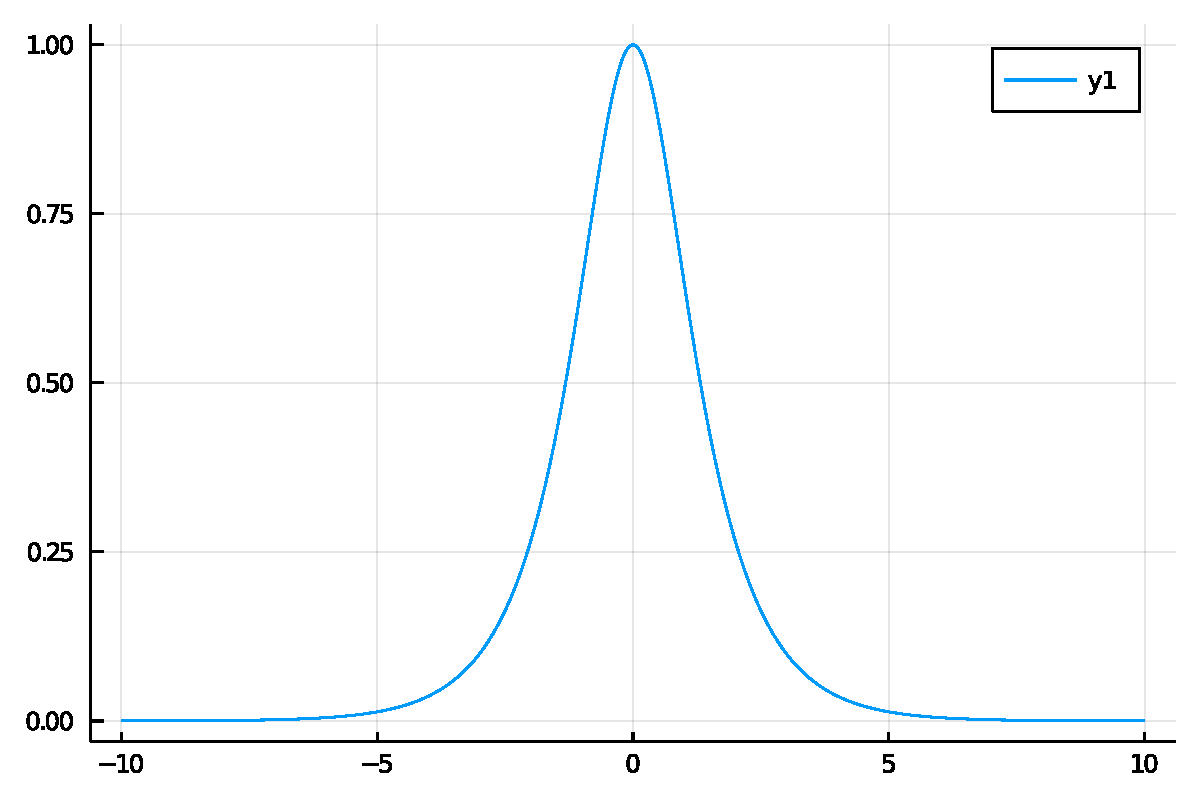
\includegraphics[width=\linewidth]{C:/Users/mfaso/OneDrive/Documents/GitHub/M3M6AppliedComplexAnalysis/output/figures/Lecture25_1_1.pdf}

Now the Fourier transform of $\sech x$ is

\[
\FF\sech(s) = \int_{-\infty}^\infty \sech t \, \E^{-\I s t} \dt = \pi \sech{\pi s \over 2}
\]
This is calculated via Residue theorem with a bit of work. Note that

\[
\pi \sech {\pi z \over 2} = {2 \pi \over \E^{\pi z \over 2} + \E^{-{\pi z \over 2}}}
\]
is analytic for $-1 < \Im z < 1$.


\begin{lstlisting}
(*@\HLJLnf{phaseplot}@*)(*@\HLJLp{(}@*)(*@\HLJLoB{-}@*)(*@\HLJLnfB{3..3}@*)(*@\HLJLp{,}@*) (*@\HLJLoB{-}@*)(*@\HLJLnfB{3..3}@*)(*@\HLJLp{,}@*) (*@\HLJLn{z}@*) (*@\HLJLoB{->}@*) (*@\HLJLn{\ensuremath{\pi}}@*)(*@\HLJLoB{*}@*)(*@\HLJLnf{sech}@*)(*@\HLJLp{(}@*)(*@\HLJLn{\ensuremath{\pi}}@*)(*@\HLJLoB{*}@*)(*@\HLJLn{z}@*)(*@\HLJLoB{/}@*)(*@\HLJLni{2}@*)(*@\HLJLp{))}@*)
\end{lstlisting}

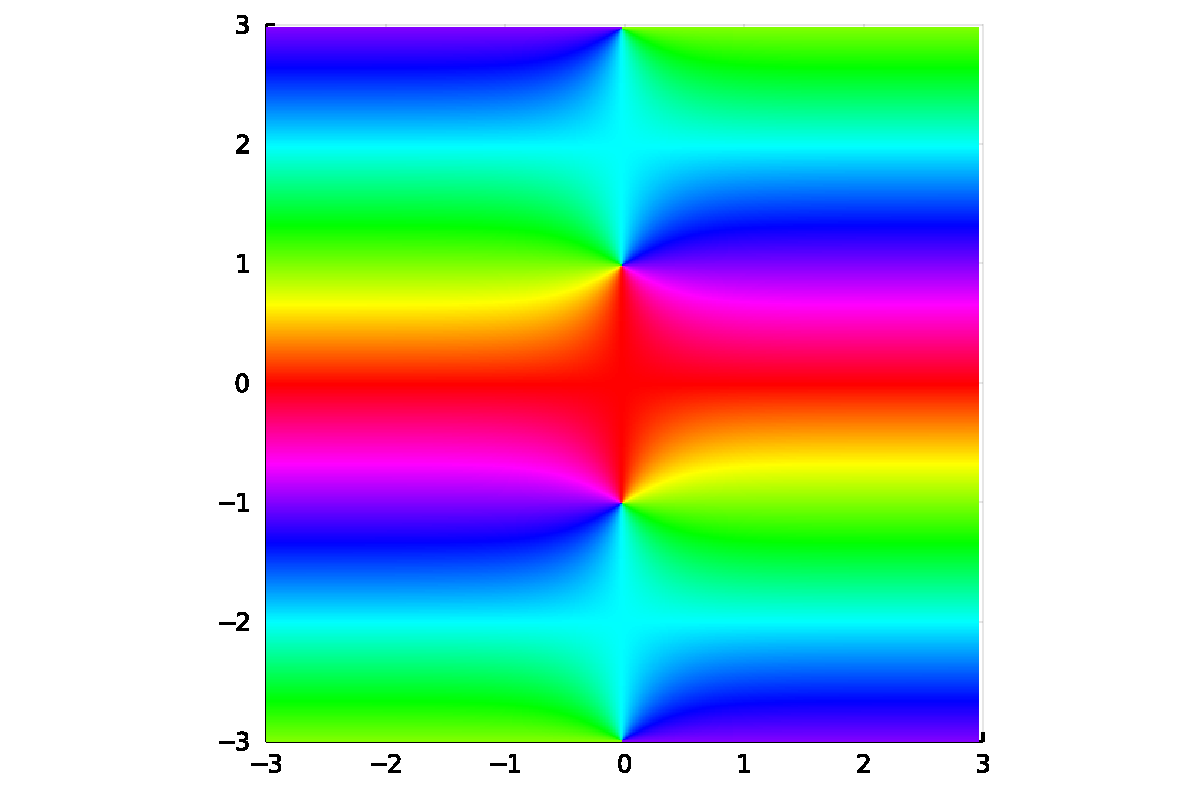
\includegraphics[width=\linewidth]{C:/Users/mfaso/OneDrive/Documents/GitHub/M3M6AppliedComplexAnalysis/output/figures/Lecture25_2_1.pdf}

This is because of the expontial decay.

\textbf{Theorem (Analyticity of Fourier transforms)} Suppose $|f(x) \E^{\gamma x}| < |M(x)|$ where $M$ is absolutely integrable for all $a < \gamma < b$. Then

\[
\widehat f(z) = \int_{-\infty}^\infty f(t) \E^{-\I z t} \dt
\]
is analytic for $a < \Im z < b$.

\textbf{Proof} Let $z = s + \I \gamma$ and note that $|f(t) \E^{-\I z t}| = |f(t) \E^{\gamma t}|$. Thus for $a < \gamma < b$, we can exchange differentiation and integration to get

\[
{\D \widehat f \over \dz} = -\I z \hat f(z)
\]
\ensuremath{\blacksquare}

\textbf{Remark} We don't need $f$ to be analytic at all!  Decay in $f$ gives analyticity.

In the case of $\sech x$, we get exponential decay in both directions: that is $\sech x \E^{|\gamma| x}$ is absolutely integrable for $\gamma < 1$.

Another example is $\E^{-x^2/2}$, which is absolutely integrable for any $\gamma$. Therefore, it's Fourier transform is in fact entire:

\[
\FF[\E^{-\diamond^2/2}](z) = \sqrt{2\pi} \E^{-{z^2 \over 2}}
\]
\subsubsection{Inverse Fourier transform on shifted contours}
A neglected fact of the Fourier transform is that we can think of $\hat f(z)$ living on any line $(-\infty + \I \gamma, \infty+\I \gamma)$, and in fact we can recover $f$ from the Fourier transform only on this line. This works even if $\hat f(s)$ is not defined on the real-axis, the real-axis is NOT special!

\textbf{Theorem} Suppose $f(x) \E^{\gamma x}$ is square integrable. Then

\[
f(x) = {1 \over 2 \pi} \int_{-\infty+\I \gamma}^{\infty + \I \gamma} \widehat f(\zeta) \E^{\I x \zeta} \D \zeta
\]
\textbf{Proof}  Note for $g(x) = f(x) \E^{\gamma x}$

\[
\widehat g(s) = \int_{-\infty}^\infty f(t) \E^{\gamma t - \I s t} \dt = \widehat f(s + \I \gamma).
\]
Therefore we have


\begin{align*}
\E^{\gamma x} f(x) &= g(x) = \FF^{-1} \widehat g(x) = {1 \over 2 \pi} \int_{-\infty}^{\infty} \widehat g(s) \E^{\I x s} \D s  ={1 \over 2 \pi} \int_{-\infty}^{\infty} \widehat f(s + \I \gamma) \E^{\I x s} \D s \\
   & = {1 \over 2 \pi} \int_{-\infty+ \I \gamma}^{\infty+ \I \gamma} \widehat f(\zeta) \E^{\I x (\zeta - \I \gamma)} \D \zeta \\
    &= {1 \over 2 \pi}
   \E^{\gamma x}  \int_{-\infty+ \I \gamma}^{\infty+ \I \gamma} \widehat f(\zeta) \E^{\I x \zeta} \D \zeta
\end{align*}
Which shows the result by cancelling out $\E^{\gamma x}$.

\subsection{Half-Fourier transforms}
Consider now

\[
\int_0^\infty f(t) \E^{-\I s t} \dt
\]
This is in fact the Fourier transform of $f$ extended to the negative real axis by zero:

\[
\int_{-\infty}^\infty \begin{cases}f(t) & t \geq 0 \\ 0 & \hbox{otherwise} \end{cases} \E^{-\I s t} \dt
\]
To make sure we remember the domain of definition, we introduce the notation:

\[
f_{\rm R}(x) = \begin{cases}f(t) & t \geq 0 \\ 0 & \hbox{otherwise} \end{cases}
\]
and

\[
f_{\rm L}(x) = \begin{cases}f(t) & t < 0 \\ 0 & \hbox{otherwise} \end{cases}
\]
Therefore

\[
\widehat\fR(s) = \int_0^\infty f(t) \E^{-\I s t} \dt \qqand \widehat\fL(s) = \int_{-\infty}^0 f(t) \E^{-\I s t} \dt
\]
Because it is identically zero on the negative real axis, we immediately get the following:

\textbf{Corollary (analyticity of Half-Fourier transform)}  Suppose $f(x)$ is bounded for $x \geq 0$. Then $\widehat{\fR}(z)$ is analytic in the lower half plane

\[
\H_+ = \{ z : \Im z < 0 \}.
\]
More generally, $f$ can even have exponential decay: if $f(x) \E^{\gamma x}$ is bounded then $\widehat\fR(z)$ is analytic in $\{z : \Im z < \gamma \}$.  As before, the same inversion formula follows:

\textbf{Corollary  (inverting Half-Fourier transform)}  Suppose  $f(x) \E^{\gamma x}$ is square integrable for $x \geq 0$. Then

\[
f(x) = {1 \over 2 \pi} \int_{-\infty + \I M}^{\infty + \I M} \widehat{\fR}(\zeta) \E^{\I x \zeta} \D \zeta
\]
for any choice of $-\infty < M \leq \gamma$.

\textbf{Example} Consider $f(x)  = x \E^{-x}$ for $0 \leq x < \infty$.  Note that $f(x) \E^{\gamma x}$ is square integrable for any $\gamma < 1$, and we have

\[
\widehat\fR(z) = \int_0^\infty t \E^{-t -\I z t} \dt = {1 \over (1+\I z)^2} = -{1 \over (z - \I)^2} 
\]
is analytic for $\Im z < 1$. Thus for any $M < 1$ we have


\begin{align*}
f(x) &= {1 \over 2 \pi} \int_{-\infty+\I M}^{\infty +\I M}\widehat\fR(\zeta) \E^{\I x \zeta}\D \zeta \\
     &={1 \over 2 \pi} \int_{-\infty+\I M}^{\infty +\I M}{1 \over (1+\I \zeta)^2} \E^{\I x \zeta}\D \zeta
\end{align*}
Since $x > 0$, we can use Residue calculus in the upper-half plane, which confirms the result:

\[
\Res_{z = \I} {\E^{\I x z} \over  (1+\I z)^2}  = \Res_{z = \I} {\E^{- x} + \I x \E^{-x} (z - \I) + O(z-\I)^2 \over  -(z-\I)^2}  = -\I x \E^{-x}.
\]
\textbf{Example} Consider $f(x) = x$.  This function is not square-integrable, but we have $f(x) \E^{\gamma x}$ is square integrable for any $\gamma < 0$, and we find for $\Im z < 0$

\[
\widehat{\fR}(z) = -{1 \over z^2}
\]
Thus we can still use the result to say, for any $M < 0$,

\[
f(x) =-{1 \over 2 \pi} \int_{-\infty+\I M}^{\infty +\I M} {1 \over \zeta^2} \E^{\I x \zeta}\D \zeta
\]
Note that the results have corresponding analogues for $\fL$:

\textbf{Corollary (analyticity of left Half-Fourier transform)} Suppose $f(x) \E^{\gamma x}$  is bounded for $x \leq 0$. Then $\widehat{\fL}(z)$ is analytic for $\{z : \Im z > \gamma \}$.

\textbf{Corollary  (inverting left Half-Fourier transform)} Suppose $f(x) \E^{\gamma x}$ is square integrable for $x < 0$. Then

\[
f(x) = {1 \over 2 \pi} \int_{-\infty + \I M}^{\infty + \I M} \widehat{\fL}(\zeta) \E^{\I x \zeta} \D \zeta
\]
for any choice of $\gamma \leq M < \infty$.

\subsubsection{Laplace transforms}
Now consider the Laplace transform

\[
\check f(z) = \int_0^\infty f(t) \E^{-z t} \dt
\]
but this is just the half Fourier transform evaluated on the negative imaginary axis!

\[
\check f(z) = \widehat\fR (-\I z)
\]
Thus if $f(x) \E^{\gamma x}$ is square integrable, then $\check f(z)$ is well-defined for $\Re z \geq \gamma$.

\emph{NEVER} think of the Laplace transform as a real-valued object: it only makes sense as a complex object. This is seen from the inverse Laplace transform

\[
f(x) = {1 \over 2 \pi \I} \int_{-\I \infty - M}^{\I \infty - M}  \check f(\zeta) \E^{\zeta x} \D \zeta
\]
which is of course just the inverse Fourier transform in disguise.

\subsection{Application: solving differential equations on the half-line}
Consider the following ODE for $x \geq 0$:


\begin{align*}
u''(x) + 2u'(x) + u(x) = f(x)
\end{align*}
with initial conditions $u(0) = u'(0) = 0$. Note that we have by integration-by-parts


\begin{align*}
\check{u'}(z) = \int_0^\infty u'(t) \E^{-z t} \dt = u(0) + z \int_0^\infty u(t) \E^{-z t} \dt = u(0) + z \check u(z) \\
\check{u''}(z) = u'(0) + z \check{u'}(z) = u'(0) + z u(0) + z^2 \check u(0)
\end{align*}
Thus taking into account the initial conditions, are equation in Laplace space becomes

\[
(z^2 + 2z + 1) \check u(z) = \check f(z)
\]
Hence we have

\[
\check u(z) = {1 \over 2 \pi \I}\int_{-\I\infty-M}^{\I \infty-M} {\check f(\zeta) \over \zeta^2 + 2\zeta+1} \E^{x \zeta} \D \zeta
\]
Consider the case $f(x) = x$, so that

\[
\check f(z) = {1 \over z^2}
\]
Here we need $M < 0$ hence we are integrating on a contour in the right-half plane.  Using Residue calculus, we have


\begin{align*}
u(x) &= \left(\Res_{z = -1} + \Res_{z=0}\right) {\E^{z x} \over z^2 (z +1)^2} \\
&= \Res_{z = -1}  {\E^{-x} +\E^{-x}(x+2) (z+1) +O(z+1)^2 \over  (z +1)^2} + \Res_{z=0} {1 + (x-2) z +O(z)^2 \over  z^2}  \\
 &= (x+2)\E^{-x} + x-2
 \end{align*}
\subsection{Laplace transform of rational functions}
We now consider the question of calculating Laplace transforms (or equivalently, half-Fourier transforms)

\[
\check f(s) = \int_0^\infty f(t) \E^{-s t} \D t
\]
where $f$ is rational. We're going to do something seemingly crazy: we'll first calculate the Cauchy transform

\[
\CC[f \E^{-s \diamond}](z) = {1 \over 2 \pi \I} \int_0^\infty {f(t) \E^{-s t} \over t- z} \D t
\]
so that

\[
\check f(s) = -2 \pi \I\lim_{z \rightarrow \infty}  z \CC[f \E^{-s \diamond}](z)
\]
Note that the exponential decay in the integrand allows us to use Plemelj's lemma: if we find a function $\phi(z)$ such that

\begin{itemize}
\item[1. ] \[
\phi(z)
\]
is analytic off $[0,\infty)$


\item[2. ] \[
\lim_{z \rightarrow \infty} \phi(z) = 0
\]
for any angle of approach


\item[3. ] \[
\phi
\]
has weaker than pole singularities at 0


\item[4. ] \[
\phi_+(x) - \phi_-(x) = f(x) \E^{-s x}
\]
\end{itemize}
Then we have calculated the Cauchy transform:

\[
\phi(z) = \CC[f \E^{-s \diamond}](z).
\]
Let's start with $f(x) = 1$ and $s = 1$, that is, what is the Cauchy transform of $\E^{-x}$? Consider the exponential integral:

\[
{\rm Ei}(z) = \int_{-\infty}^z {\E^\zeta \over \zeta} \D \zeta
\]
Without loss of generality, the contour of integration is

\[
(\infty,-1) \cup [-1, z)
\]
that is, a straight line to $-1$ and a straightline from $-1$ to $z$. Thus we have a branch cut on $[0,\infty)$ which has the jump

\[
{\rm Ei}^+(x) - {\rm Ei}^-(x) = -\oint {\E^\zeta \over \zeta} \D \zeta = -2 \pi \I
\]
where

\[
{\rm Ei}^\pm(x) = \lim_{\epsilon \rightarrow 0} {\rm Ei}(x\pm\I \epsilon)
\]
Consider

\[
\phi(z) = -{\E^{-z} {\rm Ei}(z) \over 2 \pi \I }
\]
\begin{itemize}
\item[1. ] This is analytic off $[0,\infty)$


\item[2. ] Integrating by parts we have decay at $\infty$ in all directions:

\end{itemize}
\[
\E^{-z} {\rm Ei}(z) = {1  \over z}  - \int_{-\infty}^z {\E^{\zeta-z} \over \zeta^2} \D \zeta = O(z^{-1})
\]
\begin{itemize}
\item[3. ] \[
\phi
\]
has a logarithmic singularity at 0


\item[4. ] \end{itemize}
\[
\phi_+(x) - \phi_-(x) = \E^{-x}.
\]
Thus

\[
\CC[ \E^{-s \diamond}](z) = \phi(s z) = - {\E^{-s z} {\rm Ei}(s z)  \over 2 \pi \I}
\]
Let's make sure I didn't make a mistake. Here we first define Ei:


\begin{lstlisting}
(*@\HLJLkd{const}@*) (*@\HLJLn{ei\ensuremath{\_-}\ensuremath{\_1}}@*) (*@\HLJLoB{=}@*) (*@\HLJLk{let}@*) (*@\HLJLn{\ensuremath{\zeta}}@*) (*@\HLJLoB{=}@*) (*@\HLJLnf{Fun}@*)(*@\HLJLp{(}@*)(*@\HLJLoB{-}@*)(*@\HLJLni{50}@*) (*@\HLJLoB{..}@*) (*@\HLJLoB{-}@*)(*@\HLJLni{1}@*)(*@\HLJLp{)}@*)
    (*@\HLJLnf{sum}@*)(*@\HLJLp{(}@*)(*@\HLJLnf{exp}@*)(*@\HLJLp{(}@*)(*@\HLJLn{\ensuremath{\zeta}}@*)(*@\HLJLp{)}@*)(*@\HLJLoB{/}@*)(*@\HLJLn{\ensuremath{\zeta}}@*)(*@\HLJLp{)}@*)
(*@\HLJLk{end}@*)
(*@\HLJLk{function}@*) (*@\HLJLnf{ei}@*)(*@\HLJLp{(}@*)(*@\HLJLn{z}@*)(*@\HLJLp{)}@*)
    (*@\HLJLn{\ensuremath{\zeta}}@*) (*@\HLJLoB{=}@*) (*@\HLJLnf{Fun}@*)(*@\HLJLp{(}@*)(*@\HLJLnf{Segment}@*)(*@\HLJLp{(}@*)(*@\HLJLoB{-}@*)(*@\HLJLni{1}@*) (*@\HLJLp{,}@*) (*@\HLJLn{z}@*)(*@\HLJLp{))}@*)
    (*@\HLJLn{ei\ensuremath{\_-}\ensuremath{\_1}}@*) (*@\HLJLoB{+}@*) (*@\HLJLnf{sum}@*)(*@\HLJLp{(}@*)(*@\HLJLnf{exp}@*)(*@\HLJLp{(}@*)(*@\HLJLn{\ensuremath{\zeta}}@*)(*@\HLJLp{)}@*)(*@\HLJLoB{/}@*)(*@\HLJLn{\ensuremath{\zeta}}@*)(*@\HLJLp{)}@*)
(*@\HLJLk{end}@*)

(*@\HLJLn{\ensuremath{\varphi}}@*) (*@\HLJLoB{=}@*) (*@\HLJLp{(}@*)(*@\HLJLn{z}@*)(*@\HLJLp{)}@*) (*@\HLJLoB{->}@*) (*@\HLJLoB{-}@*)(*@\HLJLnf{exp}@*)(*@\HLJLp{(}@*)(*@\HLJLoB{-}@*)(*@\HLJLn{z}@*)(*@\HLJLp{)}@*)(*@\HLJLoB{*}@*)(*@\HLJLnf{ei}@*)(*@\HLJLp{(}@*)(*@\HLJLn{z}@*)(*@\HLJLp{)}@*)(*@\HLJLoB{/}@*)(*@\HLJLp{(}@*)(*@\HLJLni{2}@*)(*@\HLJLn{\ensuremath{\pi}}@*)(*@\HLJLoB{*}@*)(*@\HLJLn{im}@*)(*@\HLJLp{)}@*)
\end{lstlisting}

\begin{lstlisting}
(*@{{\#}}@*)3 (generic function with 1 method)
\end{lstlisting}


The expression matches the Cauchy transform:


\begin{lstlisting}
(*@\HLJLn{t}@*) (*@\HLJLoB{=}@*) (*@\HLJLnf{Fun}@*)(*@\HLJLp{(}@*)(*@\HLJLni{0}@*) (*@\HLJLoB{..}@*) (*@\HLJLni{50}@*)(*@\HLJLp{)}@*)
(*@\HLJLn{s}@*) (*@\HLJLoB{=}@*) (*@\HLJLnfB{2.0}@*)
(*@\HLJLn{z}@*) (*@\HLJLoB{=}@*) (*@\HLJLnfB{2.0}@*)(*@\HLJLoB{+}@*)(*@\HLJLnfB{2.0}@*)(*@\HLJLn{im}@*)
(*@\HLJLnf{sum}@*)(*@\HLJLp{(}@*)(*@\HLJLnf{exp}@*)(*@\HLJLp{(}@*)(*@\HLJLoB{-}@*)(*@\HLJLn{s}@*)(*@\HLJLoB{*}@*)(*@\HLJLn{t}@*)(*@\HLJLp{)}@*)(*@\HLJLoB{/}@*)(*@\HLJLp{(}@*)(*@\HLJLn{t}@*)(*@\HLJLoB{-}@*)(*@\HLJLn{z}@*)(*@\HLJLp{))}@*)(*@\HLJLoB{/}@*)(*@\HLJLp{(}@*)(*@\HLJLni{2}@*)(*@\HLJLn{\ensuremath{\pi}}@*)(*@\HLJLoB{*}@*)(*@\HLJLn{im}@*)(*@\HLJLp{),}@*) (*@\HLJLnf{\ensuremath{\varphi}}@*)(*@\HLJLp{(}@*)(*@\HLJLn{s}@*)(*@\HLJLoB{*}@*)(*@\HLJLn{z}@*)(*@\HLJLp{)}@*)
\end{lstlisting}

\begin{lstlisting}
(0.02534853710699083 + 0.017828329563678146im, 0.02534853710699053 + 0.0178
28329563677806im)
\end{lstlisting}


We then recover the Laplace transform by taking the limit:

\[
\check 1(s) = -2 \pi \I  \lim_{z\rightarrow \infty} z \phi(s z) =
\lim_{z\rightarrow \infty} {z \over s z} = {1 \over s}
\]
What about rational $f$? Do the same trick of subtracting off the singularities. For example, consider $f(z) = 1/(z+1)$. Then

\[
{\phi(s z) - \phi(-s) \over z+1}
\]
satisfies all the necessary properties.


\begin{lstlisting}
(*@\HLJLn{t}@*) (*@\HLJLoB{=}@*) (*@\HLJLnf{Fun}@*)(*@\HLJLp{(}@*)(*@\HLJLni{0}@*) (*@\HLJLoB{..}@*) (*@\HLJLni{50}@*)(*@\HLJLp{)}@*)
(*@\HLJLn{s}@*) (*@\HLJLoB{=}@*) (*@\HLJLnfB{2.0}@*)
(*@\HLJLn{z}@*) (*@\HLJLoB{=}@*) (*@\HLJLnfB{2.0}@*)(*@\HLJLoB{+}@*)(*@\HLJLnfB{2.0}@*)(*@\HLJLn{im}@*)
(*@\HLJLn{f}@*) (*@\HLJLoB{=}@*) (*@\HLJLni{1}@*)(*@\HLJLoB{/}@*)(*@\HLJLp{(}@*)(*@\HLJLn{t}@*)(*@\HLJLoB{+}@*)(*@\HLJLni{1}@*)(*@\HLJLp{)}@*)
(*@\HLJLnf{sum}@*)(*@\HLJLp{(}@*)(*@\HLJLnf{exp}@*)(*@\HLJLp{(}@*)(*@\HLJLoB{-}@*)(*@\HLJLn{s}@*)(*@\HLJLoB{*}@*)(*@\HLJLn{t}@*)(*@\HLJLp{)}@*)(*@\HLJLoB{*}@*)(*@\HLJLn{f}@*)(*@\HLJLoB{/}@*)(*@\HLJLp{(}@*)(*@\HLJLn{t}@*)(*@\HLJLoB{-}@*)(*@\HLJLn{z}@*)(*@\HLJLp{))}@*)(*@\HLJLoB{/}@*)(*@\HLJLp{(}@*)(*@\HLJLni{2}@*)(*@\HLJLn{\ensuremath{\pi}}@*)(*@\HLJLoB{*}@*)(*@\HLJLn{im}@*)(*@\HLJLp{),}@*) (*@\HLJLp{(}@*)(*@\HLJLnf{\ensuremath{\varphi}}@*)(*@\HLJLp{(}@*)(*@\HLJLn{s}@*)(*@\HLJLoB{*}@*)(*@\HLJLn{z}@*)(*@\HLJLp{)}@*)(*@\HLJLoB{-}@*)(*@\HLJLnf{\ensuremath{\varphi}}@*)(*@\HLJLp{(}@*)(*@\HLJLoB{-}@*)(*@\HLJLn{s}@*)(*@\HLJLp{))}@*)(*@\HLJLoB{/}@*)(*@\HLJLp{(}@*)(*@\HLJLn{z}@*)(*@\HLJLoB{+}@*)(*@\HLJLni{1}@*)(*@\HLJLp{)}@*)
\end{lstlisting}

\begin{lstlisting}
(0.017439749335766613 + 0.013485355450154743im, 0.01743974933576627 + 0.013
48535545015414im)
\end{lstlisting}


Therefore,

\[
\check f(s) = -2 \pi \I  \lim_{z\rightarrow \infty} z {\phi(s z) - \phi(-s) \over z+1}  =
2 \pi \I \phi(-s) = -\E^{s} {\rm Ei}(-s)
\]

\begin{lstlisting}
(*@\HLJLnf{sum}@*)(*@\HLJLp{(}@*)(*@\HLJLnf{exp}@*)(*@\HLJLp{(}@*)(*@\HLJLoB{-}@*)(*@\HLJLn{s}@*)(*@\HLJLoB{*}@*)(*@\HLJLn{t}@*)(*@\HLJLp{)}@*)(*@\HLJLoB{*}@*)(*@\HLJLn{f}@*)(*@\HLJLp{),}@*) (*@\HLJLni{2}@*)(*@\HLJLn{\ensuremath{\pi}}@*)(*@\HLJLoB{*}@*)(*@\HLJLn{im}@*)(*@\HLJLoB{*}@*)(*@\HLJLnf{\ensuremath{\varphi}}@*)(*@\HLJLp{(}@*)(*@\HLJLoB{-}@*)(*@\HLJLn{s}@*)(*@\HLJLp{),}@*) (*@\HLJLoB{-}@*)(*@\HLJLnf{exp}@*)(*@\HLJLp{(}@*)(*@\HLJLn{s}@*)(*@\HLJLp{)}@*)(*@\HLJLoB{*}@*)(*@\HLJLnf{ei}@*)(*@\HLJLp{(}@*)(*@\HLJLoB{-}@*)(*@\HLJLn{s}@*)(*@\HLJLp{)}@*)
\end{lstlisting}

\begin{lstlisting}
(0.36132861688822454, 0.3613286168882152 + 0.0im, 0.3613286168882152)
\end{lstlisting}


}
\end{document}
